
\documentclass[conference]{IEEEtran}
\let\labelindent\relax
\usepackage{blindtext, graphicx}
\usepackage{listings}
\usepackage{framed}
\usepackage{caption}
\usepackage{graphicx}
\usepackage{subcaption}
\usepackage{float}
\usepackage{tikz, pgfplots}
\usepackage{soul}
\usepackage[ruled,vlined]{algorithm2e}


\ifCLASSINFOpdf
\else
\fi

% correct bad hyphenation here
\hyphenation{}

\usepackage{bera}% optional: just to have a nice mono-spaced font
\usepackage{listings}
\usepackage{xcolor}

\colorlet{punct}{red!60!black}
\definecolor{background}{HTML}{EEEEEE}
\definecolor{delim}{RGB}{20,105,176}
\colorlet{numb}{magenta!60!black}

\lstdefinelanguage{json}{
    basicstyle=\ttfamily\normalfont\footnotesize,
    numbers=left,
    numberstyle=\scriptsize,
    stepnumber=1,
    numbersep=9pt,
    showstringspaces=false,
    breaklines=true,
    frame=lines,
    backgroundcolor=\color{background},
    literate=
     *{0}{{{\color{numb}0}}}{1}
      {1}{{{\color{numb}1}}}{1}
      {2}{{{\color{numb}2}}}{1}
      {3}{{{\color{numb}3}}}{1}
      {4}{{{\color{numb}4}}}{1}
      {5}{{{\color{numb}5}}}{1}
      {6}{{{\color{numb}6}}}{1}
      {7}{{{\color{numb}7}}}{1}
      {8}{{{\color{numb}8}}}{1}
      {9}{{{\color{numb}9}}}{1}
      {:}{{{\color{punct}{:}}}}{1}
      {,}{{{\color{punct}{,}}}}{1}
      {\{}{{{\color{delim}{\{}}}}{1}
      {\}}{{{\color{delim}{\}}}}}{1}
      {[}{{{\color{delim}{[}}}}{1}
      {]}{{{\color{delim}{]}}}}{1},
}

\usepackage{lmodern}
\usepackage[utf8]{inputenc}
\usepackage[russian,english]{babel} % last one is the main language
\selectlanguage{english}

\newenvironment{russian}{
\begin{otherlanguage*}{russian}
}{
\end{otherlanguage*}
}

% URL
\usepackage{hyperref}
\urlstyle{tt}

% Better discription
\usepackage{enumitem}

%bib

\newcommand{\code}[1]{\texttt{#1}}

\begin{document}
%
% paper title
% can use linebreaks \\ within to get better formatting as desired
\title{Russian Collateral Censorship}


% author names and affiliations
% use a multiple column layout for up to three different
% affiliations
\author{\IEEEauthorblockN{Jesse Brizzi}
\IEEEauthorblockA{jbrizzi@cs.stonybrook.edu}
\and
\IEEEauthorblockN{Konstantin Dmitriev}
\IEEEauthorblockA{kdmitriev@cs.stonybrook.edu}
\and
\IEEEauthorblockN{Yingtao Tian}
\IEEEauthorblockA{yittian@cs.stonybrook.edu}
}

% make the title area
\maketitle


\begin{abstract}
%\boldmath
In this project we are proposing a survey of neighboring sovereign nations to modern day Russia to investigate any possible collateral censorship.
Given the socioeconomic state of some of these countries there may be limited infrastructure for Internet access, which requires their traffic to be routed through Russian territory.
Russia actively censors various websites and Internet sources based on various reasons.

\end{abstract}
% IEEEtran.cls defaults to using nonbold math in the Abstract.
% This preserves the distinction between vectors and scalars. However,
% if the journal you are submitting to favors bold math in the abstract,
% then you can use LaTeX's standard command \boldmath at the very start
% of the abstract to achieve this. Many IEEE journals frown on math
% in the abstract anyway.

% Note that keywords are not normally used for peerreview papers.
\begin{IEEEkeywords}
Collateral Censorship, Russia, Block, DPI, DNS, IP.
\end{IEEEkeywords}

% For peerreview papers, this IEEEtran command inserts a page break and
% creates the second title. It will be ignored for other modes.
\IEEEpeerreviewmaketitle



\section{Motivation}
In the summer of 2008, when Russia's mass media and telecom watchdog Roskomnadzor \footnote{Federal Service for Supervision of Communications, Information Technology and Mass Media (Russian:
\begin{russian}Федеральная служба по надзору в сфере массовых коммуникаций и связи\end{russian}
)} was re-established, the Russian Internet, or RuNet, changed  significantly. 
This Federal Service is regulated and put into motion by two laws, - ``On Protecting Children from Information Harmful to Their Health and Development''\cite{krem1} and ``On Information, Information Technology and Information Protection''\cite{krem2}. 
Both of them give judges a free hand in decision-making. As a result, a number of websites have been blocked quite chaotically, starting with opposition websites and articles, to Bitcoin communities and GitHub.

\indent Sometimes such censorship systems can case collateral censorship, or damage. 
They block access to sites from users beyond those intended to protect\cite{anon1}. 
This projects goal is to examine the effect of such possible collateral censorship to the requests that are originating from outside of Russia, with the possible extension to other countries that maintain the censoring services. 
The result of this project can be used to create a detailed analysis of collateral damage caused by different types of censoring techniques, and to potentially discover the paths at fault.

\section{Related Work}
Not a lot of research has been done in the area of the collateral censorship between networks in different countries.
Partly because the impact of Internet censorship on global Internet service is usually unintended, and the probability of getting any results is fairly small. 
However, China’s injection of forged DNS responses has been reported to cause large scale collateral damage by blocking outside traffic that traverses Chinese links \cite{anon1}. 
The analysis shows that in the most extreme case, 70\% of the open resolvers from Korea suffer collateral damage for queries to .de domains. 
Upstream filtering can also be behind traffic blockage outside of a censoring area due to ISP routing arrangements (for example, the Indian Internet filtering some users in Oman who are not able to access certain webpages \cite{iclab1}).

\section{Censorship tools}
The Russian Internet Service Providers (ISPs) and government use a number of different censorship techniques to block access to ``unwanted'' websites. 
Fig. \ref{fig:fig1} shows a chart of the most popular ones by the number of providers that maintain a particular method.
\begin{figure}[H]
    \centering
    \begin{tikzpicture}
    \begin{axis}[
        ybar,
        enlargelimits=0.15,
        legend style={at={(0.5,-0.15)},
          anchor=north,legend columns=-1},
        ylabel={\#providers},
        symbolic x coords={DPI-IP, IP, DPI-FULL, DNS},
        xtick=data,
        nodes near coords, 
    	nodes near coords align={vertical},
        x tick label style={rotate=45,anchor=east},
        xlabel={Blocking Method},
        x label style={at={(0.5,-0.25)}}
        ]
    \addplot coordinates {(DPI-IP,430) (IP,235) (DPI-FULL,125) (DNS, 155)};
    \end{axis}
    \end{tikzpicture}
    \caption{Number of providers that maintain a particular blocking method (DPI-IP - blocking using Deep Packet Inspection (DPI), that checks URL only at a specific IPs and port:80; DPI-FULL - blocking using DPI at every IP and ports; IP - blocking by IP address; DNS - DNS injection)}
    \label{fig:fig1}
\end{figure}

\section{Resources}
\indent As a main reference for blacklisted URLs, domain names, and IPs in Russia, we use lists provided by the ICLab, they are maintained specifically to test URL censoring. These lists are divided by country codes. Some websites are in English, some are in the local language and picked individually by the regional expert. They have content representing a wide range of categories:
\begin{itemize}
            \item Politics
            \item Social (sexuality, gambling, and illegal drugs and alcohol)
            \item Conflict/Security (armed conflicts, border disputes, separatist movements, and militant groups)
            \item Internet Tools (web sites that provide e-mail, Internet hosting, search, translation, Voice-over Internet Protocol (VoIP) telephone service)
\end{itemize}

\subsection{Challenges}
Manually analyzing lists of the blocked URLs for some countries we realized that some of them have the same censored websites, which, if not taking this into account, would give us wrong results - we might mistakenly think that some country is affected by the Russian collateral censorship, when in fact it has its own censorship. In order to overcome this problem, we have refiltered the list of the blocked URLs for Russia, our main list, in a way that have only unique URLs, that are blocked only in Russia. This procedure reduced the size of the Russian list down to 141 URLs. 

As a reference of the potential victims of the collateral censorship, we use telegraphy maps (Fig. \ref{fig:fig3}), and the map of the supported countries for one of the largest Russian backbone service provider (Fig. \ref{fig:fig2}), concentrating on the bordering countries. 

Also we are using VPNs provided by IP Vanish
\footnote{\url{https://www.ipvanish.com/}}

\begin{figure}[H]
    \centering
    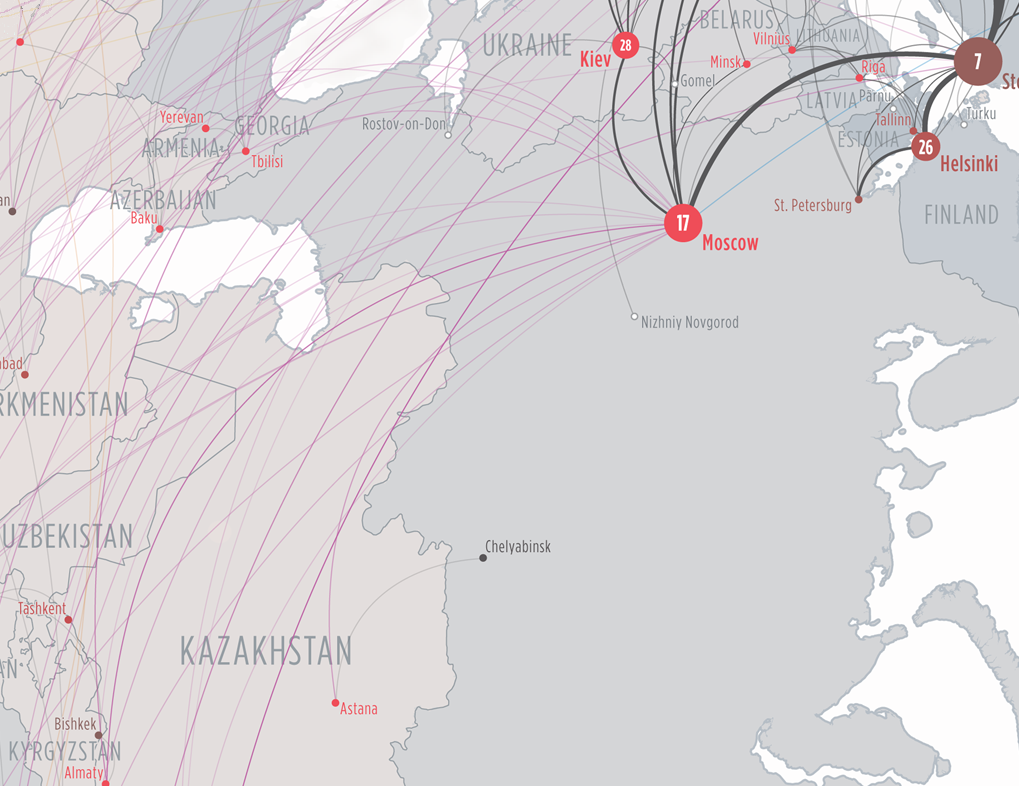
\includegraphics[width=85mm]{routeMap.png}
    \caption{Telegeography Map of the Region \label{teleG}}
    \label{fig:fig3}
\end{figure}

\begin{figure}[H]
    \centering
    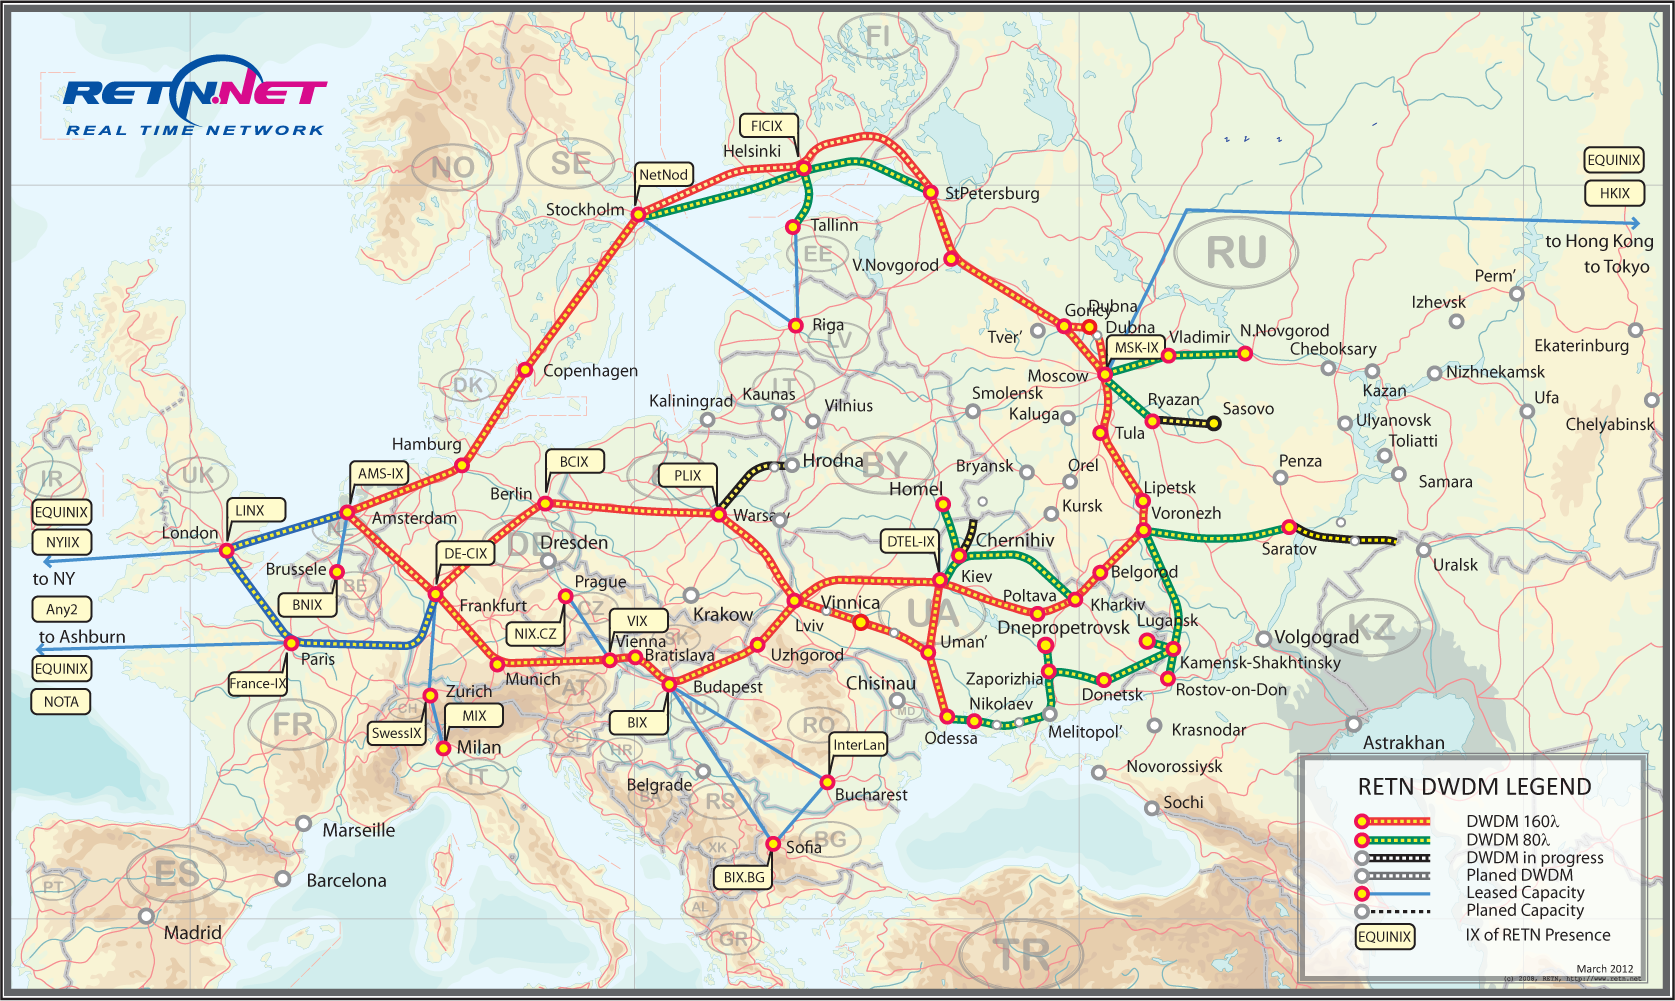
\includegraphics[width=85mm]{figure2.png}
    \caption{RETN's backbone map \label{RetnMap}}
    \label{fig:fig2}
\end{figure}


\section{Research Outline}
\subsection{Ultimate Aim}
Our ultimate aim is to write an experiment in the form of Python scripts that will probe websites censored in Russia from various points in neighboring countries. 
This experiment will not only be able to compare the received web-pages with the blocked ones, but also return the score of the similarity between the received and the blocked web-pages. 
To collect the source code of blocked web-pages we use IPVanish and ExpressVPN servers.

In order to create this experiment, we use the following modules:
\begin{enumerate}
    \item \textbf{urllib} - for network resource access;
    \item \textbf{socket} - to get an access to the BSD socket interface;
    \item \textbf{ssl} - to get an access to Transport Layer Security encryption and peer authentication facilities for network socket;
    \item \textbf{dnspython} - to get an access to high and low levels of DNS. 
\end{enumerate}
and, of course, the OpenVPN \footnote{http://openvpn.net/} client to connect to VPN servers. Also we utilize the scripts from Tunnelblick \footnote{https://code.google.com/p/tunnelblick/} for connection setup.

\subsection{Challenges}
Given the possibility where no censorship leakage is found, we will restructure the experiment to try and prove our results are accurate, i.e.\  that there is little to no collateral censorship resulting from the Russian government. 
This is done by repeating the experiment multiple times at different times of the day, along with expanding our list of candidates for possible collateral censorship to other countries in close proximity geographically and in terms of Internet topology. 

\section{Methodology}
In order to measure possible collateral damage caused by Russian censorship, we conduct an experiment that can be coarsely divided into 3 parts:
\begin{enumerate}
    \item Set a connection to a VPN server from a list of examined countries.
    \item Access and collect HTML code of web-pages that are blocked in Russia.
    \item Compare the percent of similarity between web-pages access from Russia and outside of it.
\end{enumerate}
The overall process is illustrated in Figure 4.
\begin{figure}[H]
    \centering
    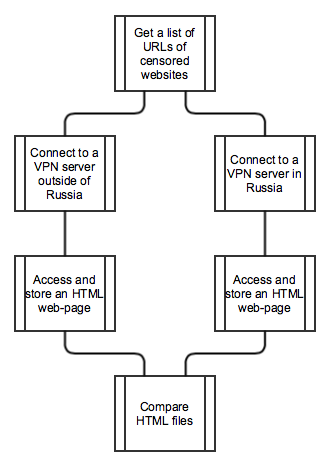
\includegraphics[width=85mm]{diag1.png}
    \caption{Scheme of the experiment \label{diag1}}
    \label{fig:fig4}
\end{figure}

\subsection{VPN}

For the connections, we are facing the following challenges:
\begin{enumerate}
    \item Access to web pages from different place, the basic need for our experiments, is required.
    \item Renting machines, either physical or virtual, is beyond our consideration, because the renting is either too expensive, or just unavailable in several countries.
    \item All communication, including data retrieval and other things like DNS request, should be done in the destination countries, because Collateral Censorship is sensitive to the path, which in turn is sensitive to DNS result.
\end{enumerate}

We are using servers provided by IPVanish and ExpressVPN because they provide access from many countries.
According to it's website \footnote{\url{https://www.ipvanish.com/why-vpn.php}}, its servers ``span 25,000+ IPs on 165+ servers in 60+ countries''.
This is a huge advantage as countries near Russia, like Finland and Estonia, are among countries supported by
IP Vanish, thus we can investigate the influence of  Russian censorship on its geographical neighbors.
Also, we are using a computer directly located in Russia to get more accurate result for Russia censorship.

For our VPN client we are using OpenVPN. 
Basically, we conntect to a OpenVPN server hosted by IP Vanish using configuration files provided by IP Vanish and associated credits.
Also we are using scripts from Tunnelblick to handle setting-up / tearing-down the connection on Mac OS X systems.
We are running OpenVPN in daemon mode, communicating with it via a telnet server open locally for management purpose.

\subsection{Data Collection}
The high-level description of the data collection algorithm is presented in pseudocode on Algorithm~\ref{algo:highlevel}.

\begin{algorithm}
        \SetAlgoLined
        Input: \textbf{ListOfCountries}, \textbf{ListOfURLs}\;
        \For{\textbf{country} in \textbf{ListOfCountries}}
        {
            Establish a connection\;
            \For{\textbf{url} in \textbf{ListOfURLs}}
            {
                Access a webpage (timeout = 2 sec)\;
                Store its HTML code\;
            }
        }
        \caption{Data Collection}
        \label{algo:highlevel}
\end{algorithm}

The algorithm goes through every country in the list of selected countries, then it establishes a VPN connection, and then requests all 141 urls from the list of blocked URLs in Russia, it accesses the webpage within 2 seconds timeout and stores it's HTML code for the offline comparison.

For the purpose of data collection we implemented a special class - \code{CollectData}. Its instance connects to a specified VPN server and performs either collection of a single wep-page, specified by a URL from multiple countries, or collects a list of web-pages, using single VPN connection (Country major vs Website major order).
This gives us the option of targeting a specific website in a small time windows to minimise differences in time sensitive content. 

We chose to collect the webpage is country major order rather than website major order because to time restrictions. 
Collecting the website in website major order would be better as it would shrink the time window that we are accessing the webpages to minimize time based differences in the webpages. 
This is inefficient in times as the vpn takes multiple seconds to connect and disconnect from the server, and if we had to do this for every webpage rather than every country the data collection portion of our project would take days rather than hours. 

After the web-page access attempt, there could be four possible outcomes:
\begin{enumerate}
    \item An original web-page.
    \item A web-page with a removed part (partial censorship,    Figure~\ref{fig:partial}).
    \item A censorship's system brochure web-page (Figure~\ref{fig:brochure}).
    \item A failure to load a web-page.
\end{enumerate}
In order to deal with the final case, we stop waiting for a response after 2 seconds (Timeout parameter).

\begin{figure}
\centering
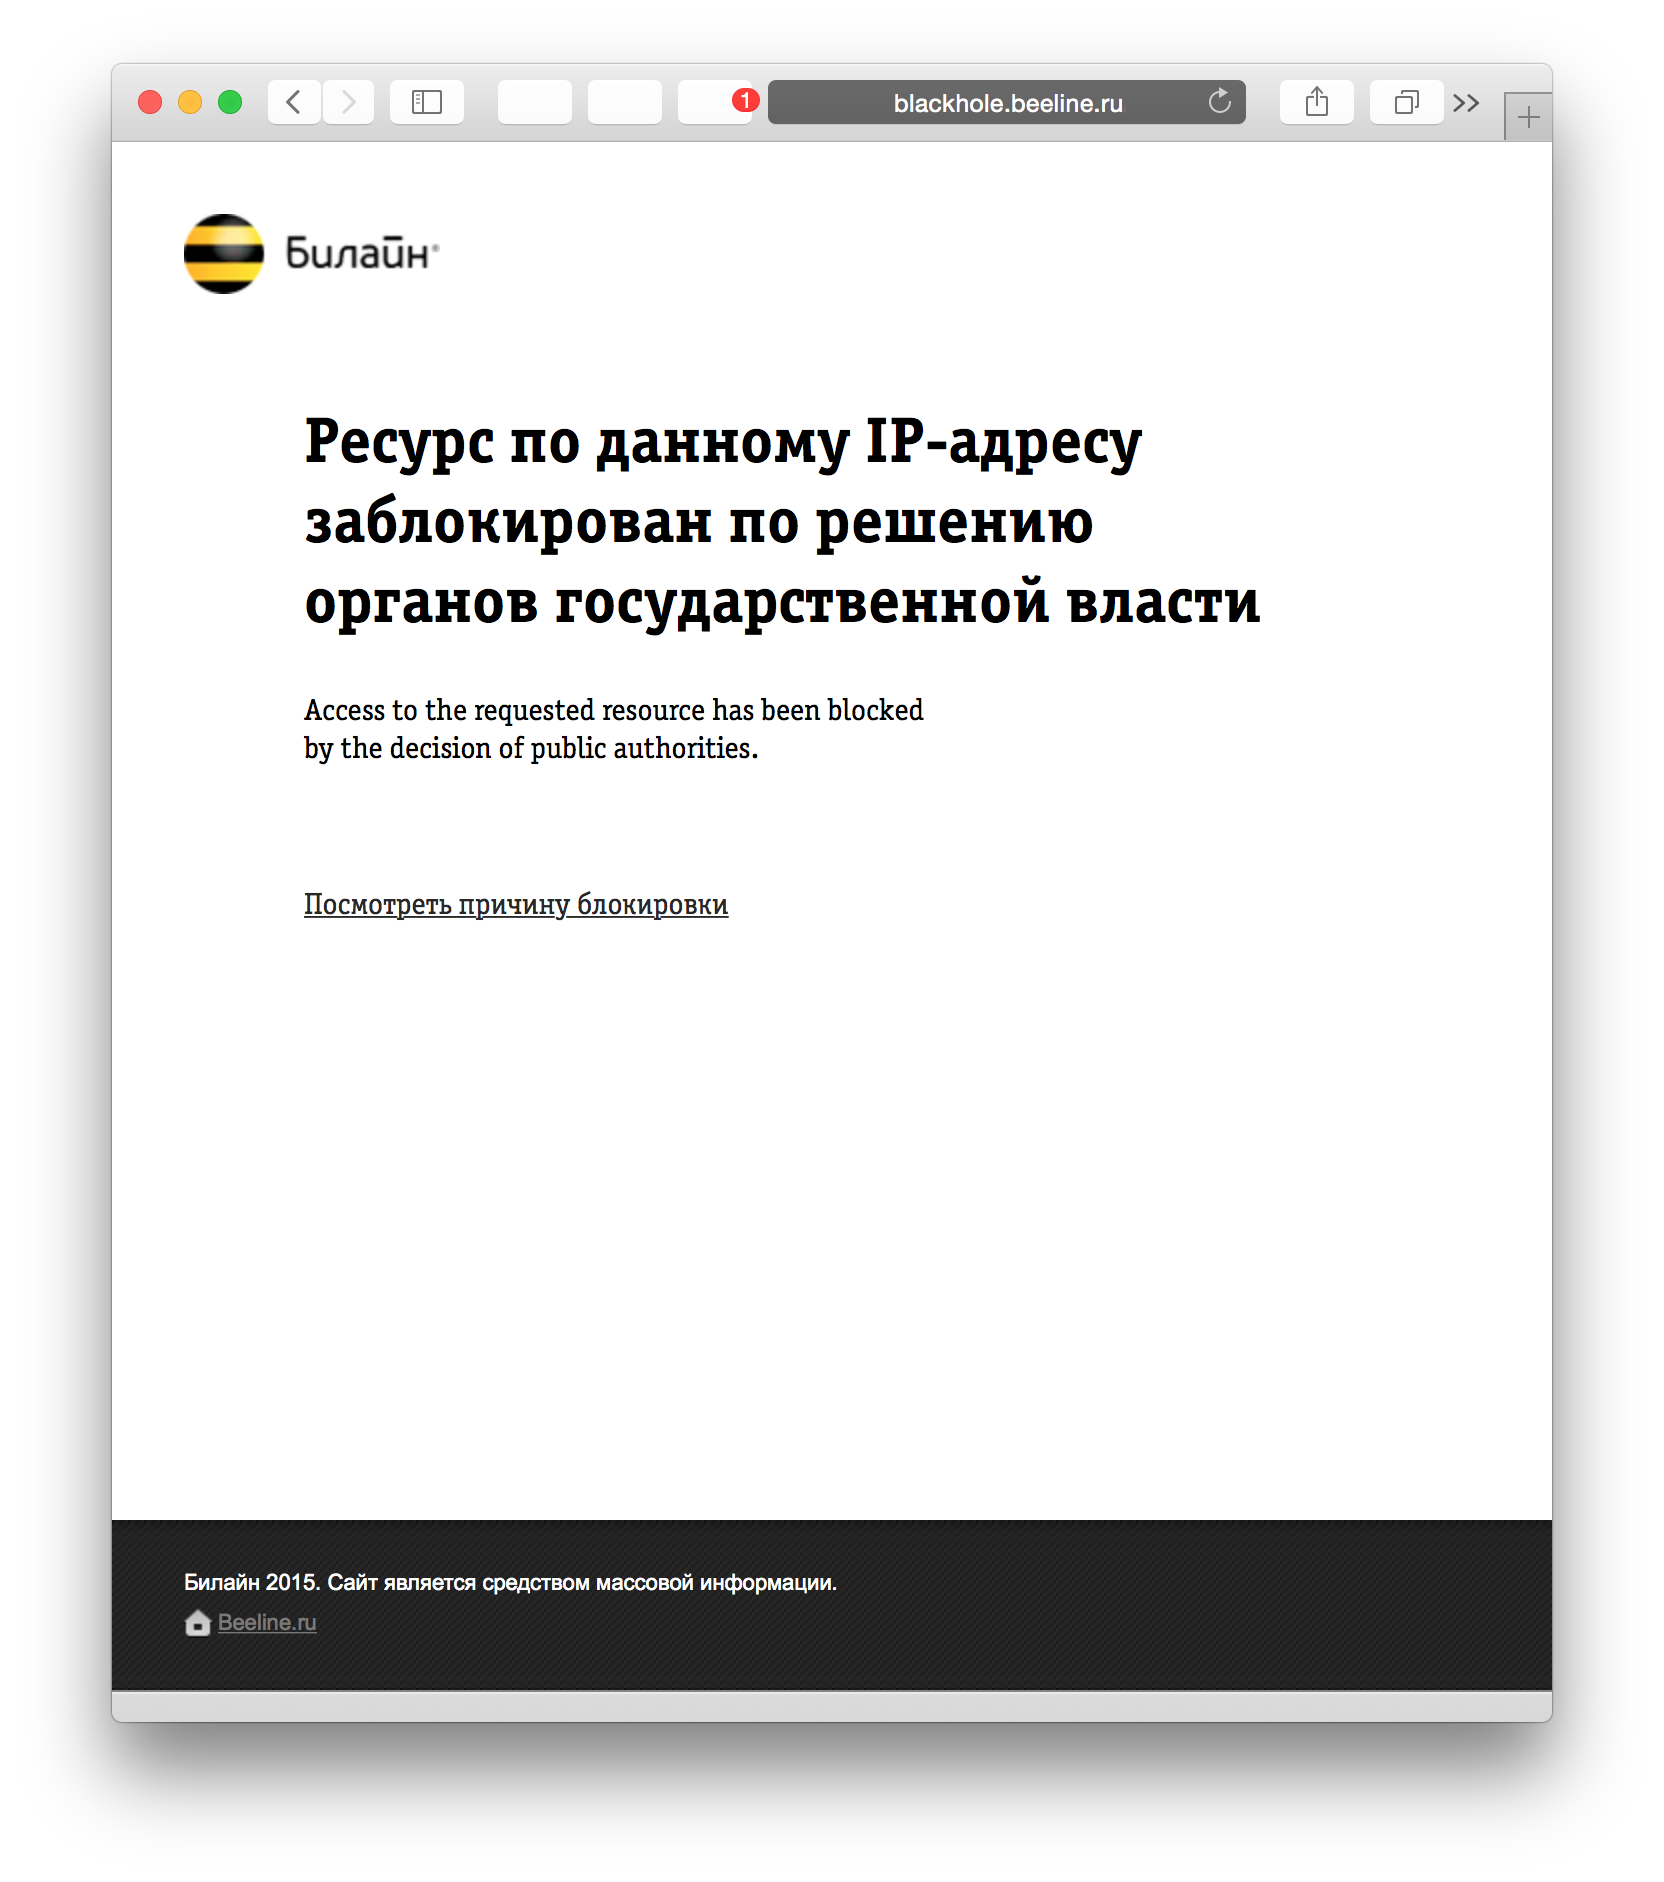
\includegraphics[width=0.3\textwidth]{azartplay-kyrgystan.png}
\caption{Example of provider's brochure page}
\label{fig:brochure}
\end{figure}

\begin{figure}
        \centering
        \begin{subfigure}{0.3\textwidth}
            \centering
            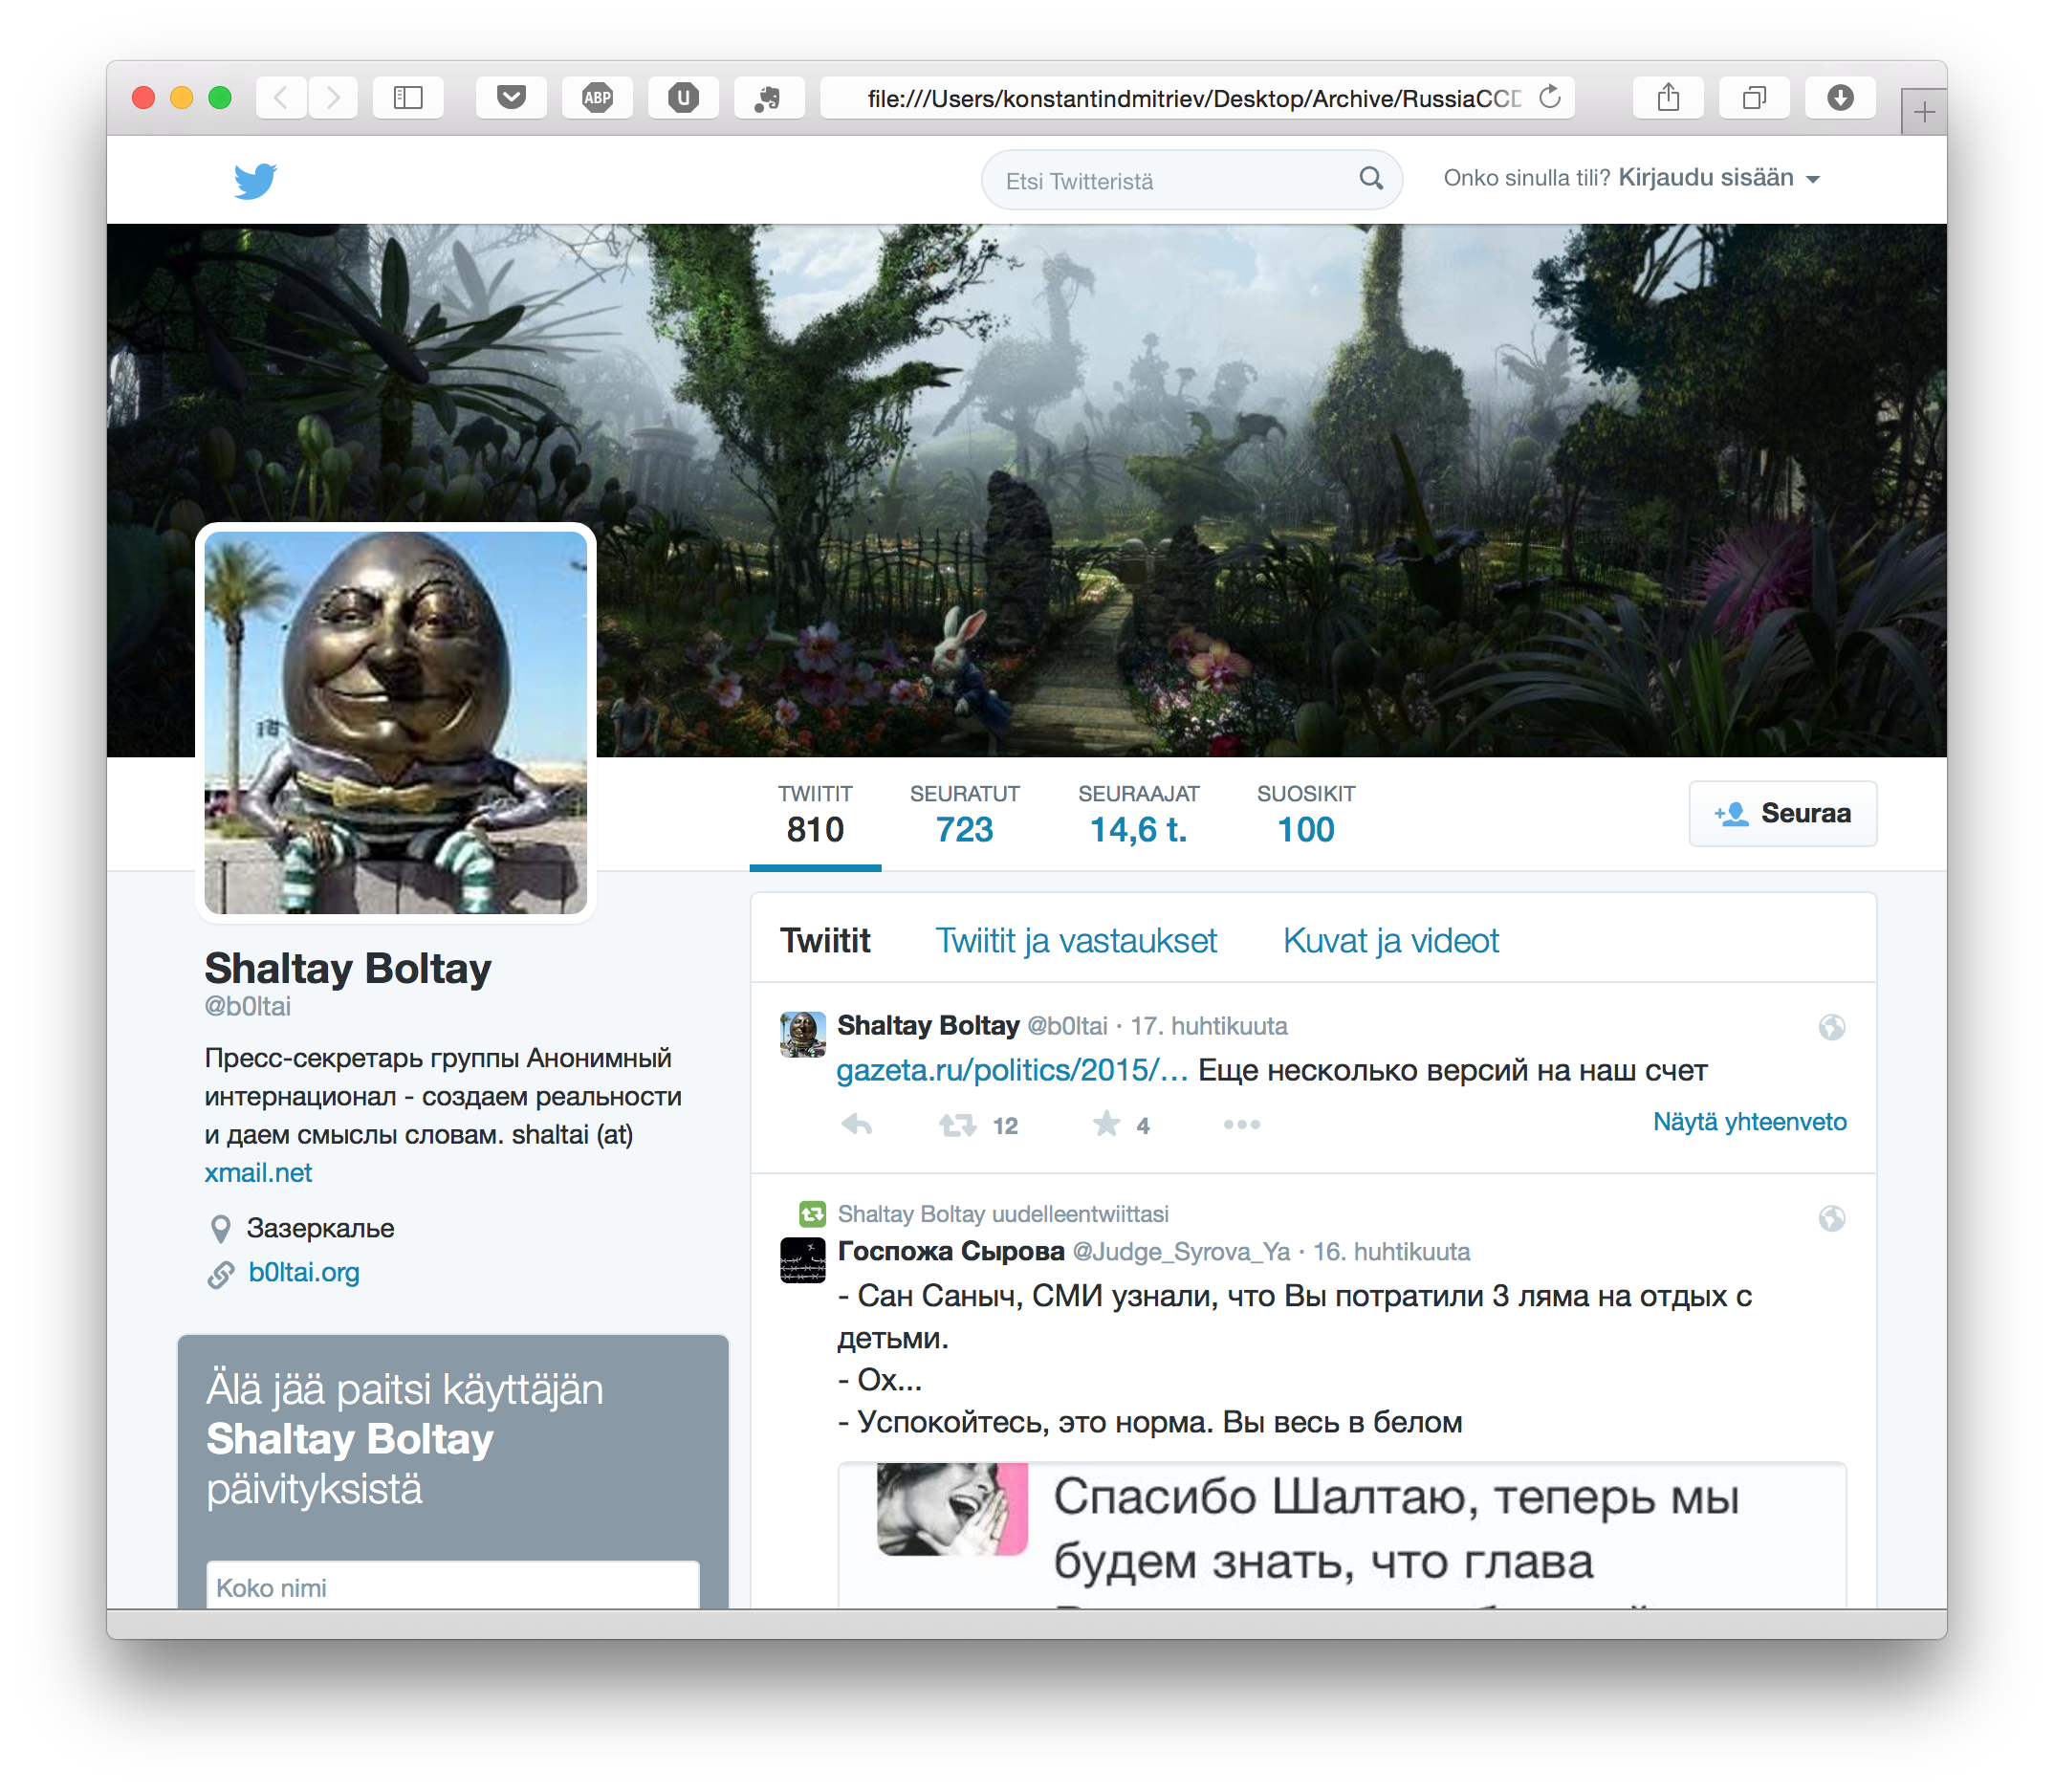
\includegraphics[width=\textwidth]{twi1.png}
            \caption{Latvia}
            \label{fig:pic1}
        \end{subfigure}
        \\
        \begin{subfigure}{0.3\textwidth}
            \centering
            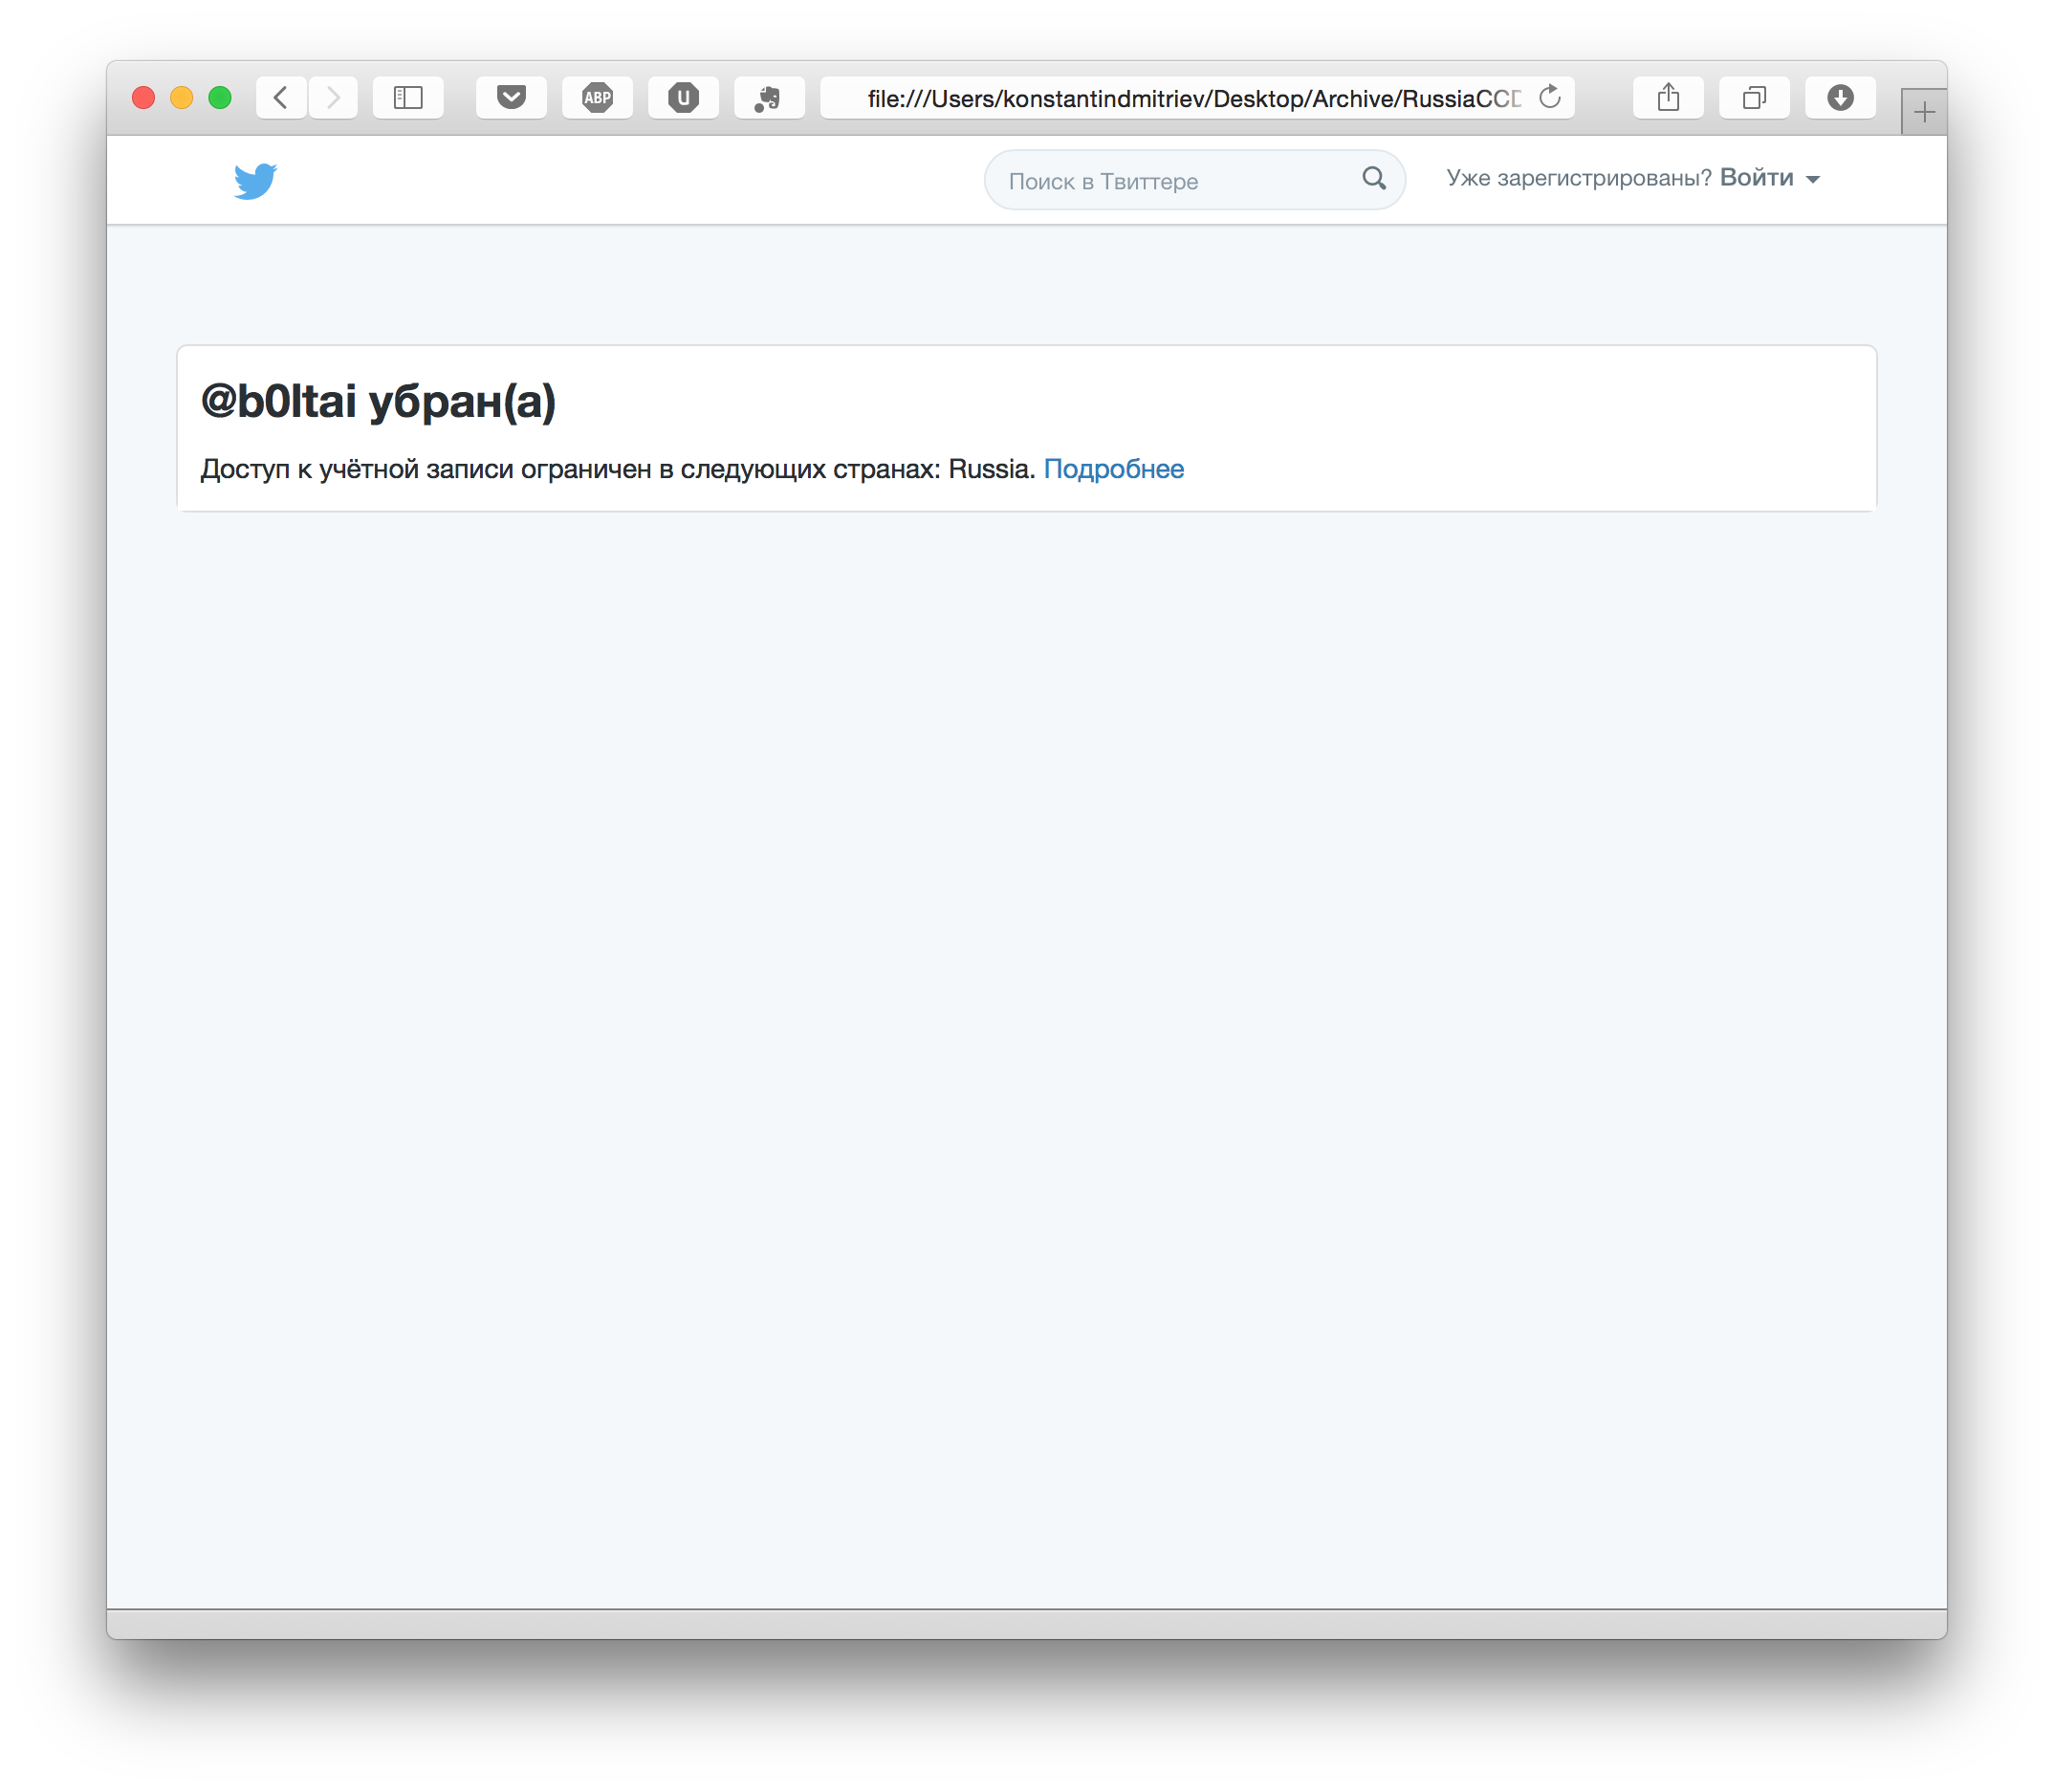
\includegraphics[width=\textwidth]{twi2.png}
            \caption{Russia}
            \label{fig:pic2}
        \end{subfigure}
        \caption{Example of the partial censorship}
        \label{fig:partial}
    \end{figure}

\subsection{Web Page Comparison}

Web Page comparison is an essential part of our project.
The aim is to compare the similarity between different copies of the same page accessed from difference countries.
Censorship usually alters the content of web pages, 
so if a pages is effected by censorship in one country,
the content varies between a copy accessed from this country,
and one from a reference uncensored country.
In this scenario, comparing the similarity
between these different copies provides us an efficient
way to detect and quantify the content changes.

However, the content changes could also happen due to reasons
besides censorship.
Some of the reasons could be temporal, 
for example a change of time stamp in these copies are totally reasonable,
while another example may be recent news blocks in some news sites.
Also valid reasons include geographical customization, 
such as local news that varies from one place to another one.

These two kinds of content changes are different:
The changes due to censorship tend to replace the whole page,
while the normal changes are more block-wise, and thus 
preserving general architecture of web pages.
Therefore, Our algorithm should be sensitive to a fully change page,
but meanwhile insensitive to  block changes, especially small ones.

\begin{algorithm}
    \SetAlgoLined
    \KwData{Two strings $S_{1\dots n}$ and $T_{1\dots m}$}
    \KwResult{Length of longest common subsequence of $S$ and $T$}
    
    $F_{0\dots n, 0\dots m} \gets 0$\;
    \For{$i\leftarrow 1$ \KwTo $n$}{
        \For{$j\leftarrow 1$ \KwTo $m$}{
            $F_{i,j} \gets \max( F_{i-1,j}, F_{i,j-1} )$\;
            \If{$S_i = T_j$}{
                $F_{i,j} \gets \max( F_{i,j}, F_{i-1,j-1}+1 )$
            }
        }
    }
    \Return $F_{n,m}$
    
    \caption{Longest Common Subsequence}
    \label{algo:lcs}
\end{algorithm}

We hereby propose the use of Longest Common Subsequence, or LCS, for scoring. LCS is a good metric for HTML file comparison, because it is relatively robust to block-wise content change (I.E a DOM tree node is replaced by another one, while preserving other parts of the tree). 
The algorithm for LCS is detailed on Algorithm~\ref{algo:lcs}.
More precisely, we use the following scoring formula:
\[ Score(s_1,s_2) = \frac{LCS(s_1,s_2)}{Len(s_1)+Len(s_2)} \]
to ensure that our similarity metric would not prefer longer/shorter web pages.
This metric means that a larger score means larger degree of similarity, also the score is constrainted in a given range ($0\leq score \leq 0.5$), so the results are comparable for all page length.

However, a plain implementation of LCS is time-consuming: 
It requires $O(n m)$ time to compute where $n$ and $m$ are lengths of two strings, respectively. This is insufficient for HTML comparison because the average size of contemporary pages has already excessed $1.6$ million bits\footnote{\url{http://www.websiteoptimization.com/speed/tweak/average-web-page/}}, 
or $200$ kilo-bytes.

\begin{algorithm}
    \SetAlgoLined
    \KwData{Two strings $S_{1\dots n}$ and $T_{1\dots m}$, and $O$, the maximum offset}
    \KwResult{Approximate length of longest common subsequence of $S$ and $T$, with respect to maximum offset $O$}
    
    \If{$n=0$ or $m=0$}{
        \Return $0$\;
    }
    $i \gets 1$\;
    $j \gets 1$\;
    $lcs \gets 0$\;
    \While{$i \leq n$ and $j \leq m$}{
        \uIf{$S_i = T_j$}{
            $lcs \gets lcs + 1$\;
        }
        \Else{
            \uIf{$i<j$}{
                $j \gets i$\;
            }
            \Else{
                $i \gets j$\;
            }
            \For{$k\gets 0$ \KwTo $O-1$}{
                \If{$i+k \leq n$ and $S_{i+k} = T_j$}{
                    $i \gets i + k$\;
                    break\;
                }
                \If{$j+k \leq m$ and $S_i = T_{j+k}$}{
                    $j \gets j + k$\;
                    break\;
                }
            }
        }
        $i \gets i + 1$\;
        $j \gets j + 1$\;
    }
    \Return $lcs$
    
    \caption{Sift3b}
    \label{algo:sift3b}
\end{algorithm}

This means that we need to use some algorithm that is more efficient.
One such algorithm we are using is Sift3b \cite{sift3b}, 
which is an approximate algorithm with speed optimizations,
as shown in Algorithm~\ref{algo:sift3b}.

Sift3b approximates the longest common subsequence by setting a parameter $O$, or max offset, and ignoring attempts to match characters whose offset is larger than the max offset.
This means the running time of Sift3b is $O( (n+m) O)$
where $n$ and $m$ are lengths of two strings, respectively.
This gives us some kind of trade-off in parameters, because a larger max offset means a better approximation and slower running time.
For our problem, we choose $O=130$ for a balance between accuracy and running time.

\section{Results}
After running the comparison algorithm and assigning every page a score, we measure the possibility of some country being affected by the collateral censorship by analyzing the data, same 141 webpages, but accessed from the USA. We ran the comparing algorithm once again, calculated the score for every page accessed from the USA, estimated the mean $\mu^{USA}$ and the standard deviation $\sigma^{USA}$. Then, we assume, that if some country has a mean value which is more than the mean value for the USA, then there is a high chance of the censorship leakage from Russia:
\[\mu^{country} > \mu^{USA} + k*\sigma^{USA} - country\ is\ affected\]\\
\[\mu^{country} \leq \mu^{USA} + k*\sigma^{USA} - country\ is\ not\ affected\]

For the final step, we've collected more than 25000 webpages, using IPVanish and ExpressVPN servers, the results are presented in Figure~\ref{fig:results}.
This bar chart shows that 4 countries (Belarus, Estonia, Lithuania and Ukraine) show some signs of the possible censorship leakage.

There is another interesting finding. We were able to detect sings of the censorship leakage only from IPVanish vantage points. The possible explanation is that ExpressVPN circumvents the censorship on its own, since that's what most of their users would want.

\begin{figure}
    \begin{tikzpicture}
    \begin{axis}[
        ybar,
        ymin=0.6,
        enlargelimits=0.15,
        legend style={at={(0.5,-0.3)},
          anchor=north,legend columns=-1},
        ylabel={Score},
        symbolic x coords={Azerbaijan, Belarus, Finland, Estonia, Georgia, Latvia, Lithuania, Ukraine, Kazakhstan, Kyrgyzstan, Mongolia, Russia, USA},
        xtick=data,
        ybar=3pt,
        bar width=1
        nodes near coords, 
    	nodes near coords align={vertical},
    	every node near coord/.append style={rotate=90, anchor=west},
        x tick label style={rotate=45,anchor=east},
        x label style={at={(0.5,-0.25)}}
        ]
    \addplot coordinates {(Azerbaijan,0) (Belarus,0.803) (Kazakhstan,0.728) (Finland,0.764) (Lithuania,0.806) (Kyrgyzstan,0.766) (Ukraine,0.814) (Latvia,0.784) (Estonia,0.8) (Russia,1.0) (Georgia,0) (Mongolia,0) (USA, 0)};
    \addplot coordinates {(Finland,0.702) (Belarus,0) (Lithuania,0.71) (Kyrgyzstan,0.735) (Ukraine,0.736) (Latvia,0.724) (Estonia,0.742) (Russia,1.0) (Kazakhstan,0.720) (Azerbaijan,0.722) (Mongolia,0.720) (Georgia,0.732) (USA, 0)};
    \addplot+[error bars/.cd,y dir=both,y explicit]
    coordinates {(USA, 0.717) +- (USA, 0.073)};
    
    \draw[very thin,red] ({rel axis cs:0,0} |- {axis cs:Belarus,0.79}) --
      ({axis cs:USA,0.79} -| {rel axis cs:1,0});

    \legend{IPVanish,ExpressVPN, Model(USA)}
    \end{axis}
    \end{tikzpicture}
    \caption{Results. Red bars are the mean values for the respective country estimated using ExpressVPN, blue bars are the mean values estimated using IPVanish. The most right bar is the mean and std values for the USA. The horizontal red line is the maximum mean value that indicates the possible collateral censorship for countries with higher scores.}
    \label{fig:results}
\end{figure}

\section{Current Issues}

A major obstacle that we plan to overcome in the future is the inconsistency of the censorship from our different viewpoints from \textit{within} Russian borders.
Using our various VPN subscriptions and a physical computer that we have access to in Russia we are observing different levels of access to certain websites.
Our PC in Russia is censored in more cases then it is not when testing against the list of target websites.
Where our VPN service through IP Vanish seems to get through to most of these websites. 
This may be due to the VPN company purposely fetching these locked websites as this would be a feature that most of its users would want or their servers are falsely labeled as being located in Moscow. 
We just happen to be in the fringe case of actually wanting to be censored.

We plan on either only collecting Russian samples from our dedicated PC or trying a difference VPN service. 
An issue may be similar de-censorship in the neighboring countries too, but we do not have dedicated machines in these locations to check. 
This may lead to a lot of invalid results in the end. 

\section{Future Work}

Currently we plan on focusing on expanding our HTML comparison methods to try and find what type of things are being changed if only parts of webpages are being censored.
To account for different dynamic content that may change from instance to instance (ads, time dependant information).

We have references to methods of figure printing the type of censorship being used from the Russian ISPs, we would like to integrate this into our project as well. 
\begin{thebibliography}{9}


\bibitem{anon1}
  Anonymous,
  \emph{The Collateral Damage of Internet Censorship by DNS Injection}.
  SIGCOMM Comput. Commun. Rev., July 2012.
  
\bibitem{krem1}
    \emph{"Law on Protecting Children from Negative and Harmful Information."} President of Russia. N.p., n.d. Web. 14 Feb. 2015. 
    
\bibitem{krem2}
    \emph{Russian Federation: Federal Law No. 149-FZ} of July 24, 2006, on Information, Information Technology and Information Protection (as Amended up to Federal Law No. 398-FZ of December 28, 2013). N.p., n.d. Web. 14 Feb. 2015.
    
\bibitem{iclab1}
C. Lab., 
    \emph{Routing Gone Wild: Documenting upstream filtering in Oman via India.} Technical report, Citizen Lab, 2012. 


\bibitem{sift3b} S. Zackwehdex, \emph{Super Fast and Accurate string distance algorithm: Sift3}, Web post, accessed at May 1,\ 2015, available at \\ \url{http://siderite.blogspot.com/2007/04/super-fast-and-accurate-string-distance.html}.

\end{thebibliography}

\end{document}
